\documentclass[handout]{beamer}

\usepackage{Haust2017glærur}

\title{Tölvunarfræði 1a}
\subtitle{Vika 13, seinni fyrirlestur}

\begin{document}

\begin{frame}
\titlepage
\end{frame}

\section{Inngangur}

\begin{frame}{Í síðasta þætti\ldots}
    \begin{itemize}
        \item Tölfræðiföll
        \item Meiri hlutbundin forritun
    \end{itemize}
\end{frame}

\section{Tímaflækjur}

\begin{frame}{Tímaflækjur}
    \begin{itemize}
        \item Tímaflækja (e. \emph{time complexity}) er lykilhugtak í tölvunarfræði
        \begin{itemize}
            \item Tímaflækja reiknirits segir til um hvernig forritið hegðar sér \emph{sem fall af inntaksstærð}
            \item Mjög einfölduð tímaflækjugreining: Gerum ráð fyrir að hver grunnaðgerð taki fastan tíma og teljum grunnaðgerðirnar
            \item Hversu margar aðgerðir þarf forrit sem tekur inntak af stærðinni $n$?
            \begin{itemize}
                \item Stærstu inntökin eru erfiðust, áhugavert er að skoða hvað gerist þegar $n \to \infty$
            \end{itemize}
        \end{itemize}
        \item Tímaflækja reiknirits er áháð keyrslutíma á ákveðinni vél 
        \begin{itemize}
            \item Gefur okkur almennari upplýsingar en þær sem við fáum með \texttt{tic} og \texttt{toc}
        \end{itemize}
    \end{itemize}
\end{frame}

\begin{frame}{Grundvallarvandamál}
    \begin{itemize}
        \item Sum vandamál koma oftar upp en önnur
        \item Tvö grundvallarvandamál:
        \begin{itemize}
            \item Leitarvandamálið
            \begin{itemize}
                \item Getum lýst því sem uppflettingu í nafnatöflu (e. \emph{symbol table})
            \end{itemize}
            \item Röðunarvandamálið
            \begin{itemize}
                \item Höfum stök sem við getum borið saman, viljum fá þau í stígandi röð
            \end{itemize}
        \end{itemize}
    \end{itemize}
\end{frame}

\begin{frame}{Hugmyndin um nafnatöflu}
    \begin{itemize}
        \item Höfum stök þar sem hvert samanstendur af lykli (e. \emph{key}) og gildi (e. \emph{value})
        \item Notum lykilinn til að fletta upp gildum
        \begin{itemize}
            \item Dæmi: Flettum upp nafni með því að nota kennitölu
        \end{itemize}
        \item Ef við notum fylki til að geyma stökin vex keyrslutíminn línulega með fjölda staka í nafnatöflunni
        \begin{itemize}
            \item Útfærsla með helmingunarleit er mun hraðvirkari þegar töflurnar eru stórar
        \end{itemize}
    \end{itemize}
\end{frame}

\begin{frame}{Helmingunarleit}
    \begin{center}
        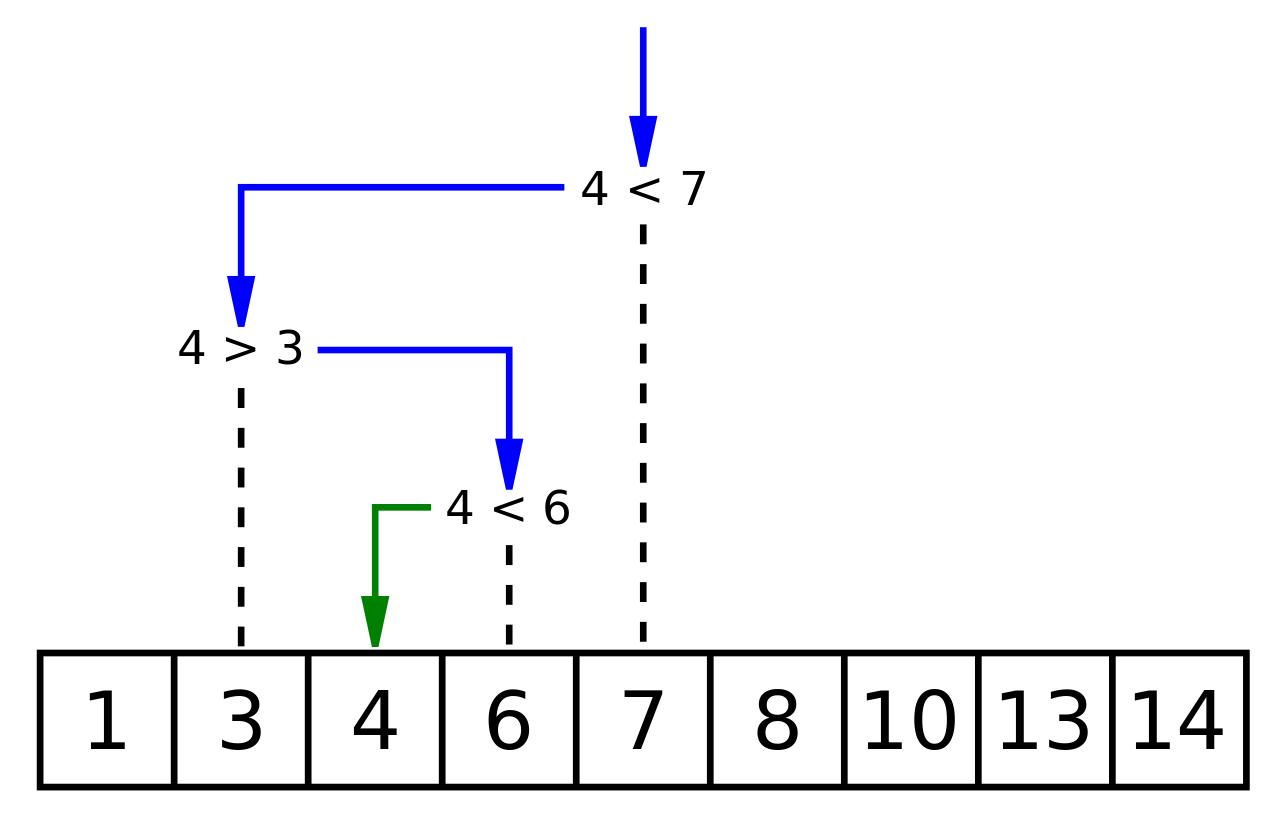
\includegraphics[width=0.7\textwidth]{bs}

        Mynd: \href{https://upload.wikimedia.org/wikipedia/commons/thumb/6/64/Binary_search_into_array_-_example.svg/1280px-Binary_search_into_array_-_example.svg.png}{Wikipedia}
    \end{center}
\end{frame}

\begin{frame}{Tvíleitartré}
    \begin{center}
        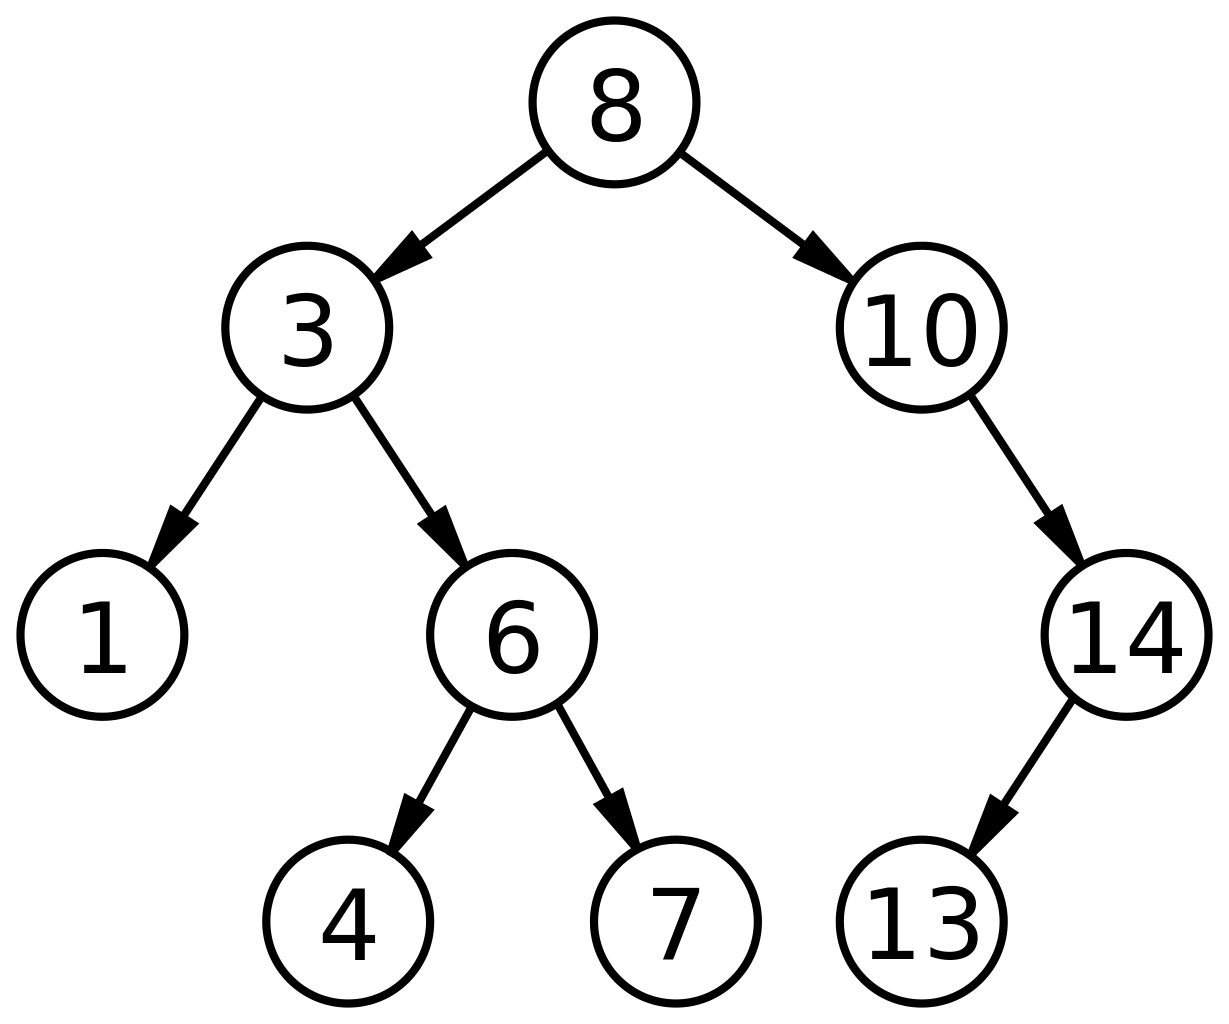
\includegraphics[width=0.6\textwidth]{bst}

        Mynd: \href{https://en.wikipedia.org/wiki/File:Binary\_search\_tree.svg}{Wikipedia}
    \end{center}
\end{frame}

\begin{frame}{Röðunarreiknirit}
    \begin{itemize}
        \item Röðunarvandamálið:
        \begin{itemize}
            \item Höfum safn af stökum, viljum fá þau í stígandi röð
            \item Í Matlab er þetta safn af stökum venjulega bara vigur
        \end{itemize}
        \item Ekki er hægt að nota samanburði til að raða $n$ stökum á tíma sem vex hægar en $n\cdot \log(n)$
        \item Í Matlab höfum við innbyggða fallið \texttt{sort} sem getur bjargað okkur
        \item Getum búið til önnur röðunarreiknirit
        \begin{itemize}
            \item Skoðum sameiningarröðun (e. \emph{Merge sort}), sem byggist á endurteknum sameiningum á smálistum
        \end{itemize}
    \end{itemize}
\end{frame}

\begin{frame}{Merge sort}
    \begin{center}
        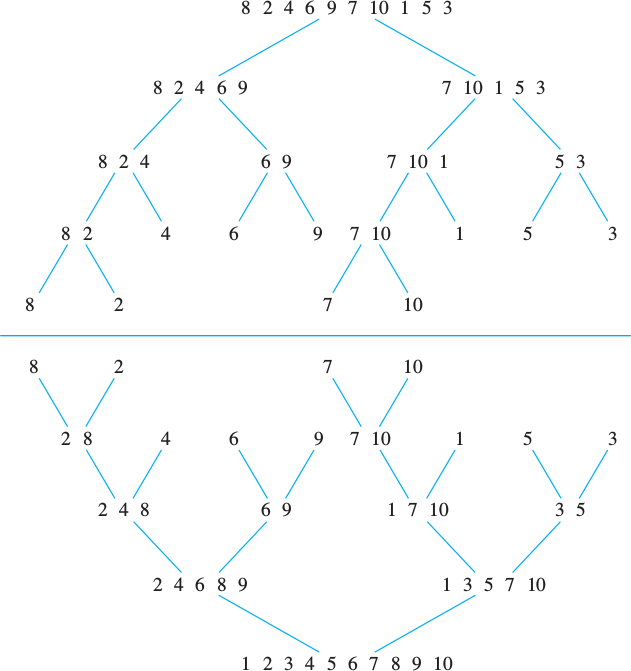
\includegraphics[width=0.5\textwidth]{merge-sort-visual}
    \end{center}
\end{frame}

\begin{frame}{Fyrirlestraræfing}
    \begin{itemize}
        \item Setja á 31 lykil inn í tvíleitartré. Hversu hátt þarf tréð að vera?
        \item Hvað þarf lykkja margar ítranir til að sameina tvo raðaða vigra, þar sem annar vigurinn er með $n$ stök en hinn $m$ stök? 
    \end{itemize}
\end{frame}

\end{document}
